\section{Ziel}
    In diesem Versuch sollen die Topologien verschiedener Strukturen im Micrometerbereich sowie die von Speicherdiscs wie CD, DVD und Blu-Ray untersucht werden. Dazu wird die Methode der \textit{atomic force
    microscopy} (AFM) verwendet, die auf der Auslenkung einer wenigen Nanometer großen Spitze aufgrund der Wechselwirkung zwischen dieser und den Oberflächenatomen basiert.    
    
\section{Theoretische Grundlagen}
    \subsection{Messprinzip}
        Das klassische Messprinzip der AFM ist in Abbildung \ref{fig:prinzip} visualisiert. Eine \textbf{Messspitze} (\textit{Probe Tip}), die an einem \textbf{Cantilever} befestigt ist, wird auf eine 
        Entfernung von wenigen Angström bis einigen \SI{100}{\nano\metre} and die Probenoberfläche gebracht. Die zwischen der Messspitze und den Oberflächenatomen wirkende Kraft resultiert aus verschiedenen
        distanzabhängigen \textbf{Wechselwirkungen} und wird auf den Cantilever übertragen. Verschiedene \textbf{Detektionssysteme} erlauben es die wirkende Kraft über den Cantilever zu messen und so den 
        Abstand zwischen Messspitze und Oberfläche zu bestimmen. In Kombination eines elektronischen Feedback-Loops und \textbf{Piezoelementen}, die die Probe relativ zur Messspitze in x-, y- und z-Richtung
        verschieben können, ist es möglich diese Abstandsmessung auf der gesamten Probe durchzuführen und so ein Höhenprofil der Oberfläche zu ermitteln. Da je nach Distanz verschiedene Kräfte dominieren und
        der Feedback-Loop es auch ermöglicht auf verschiedene Weise über die Probe zu rastern, kann die AFM in mehreren \textbf{Messmodi} betrieben werden.

        \FloatBarrier

        \begin{figure}[h]
          \centering
          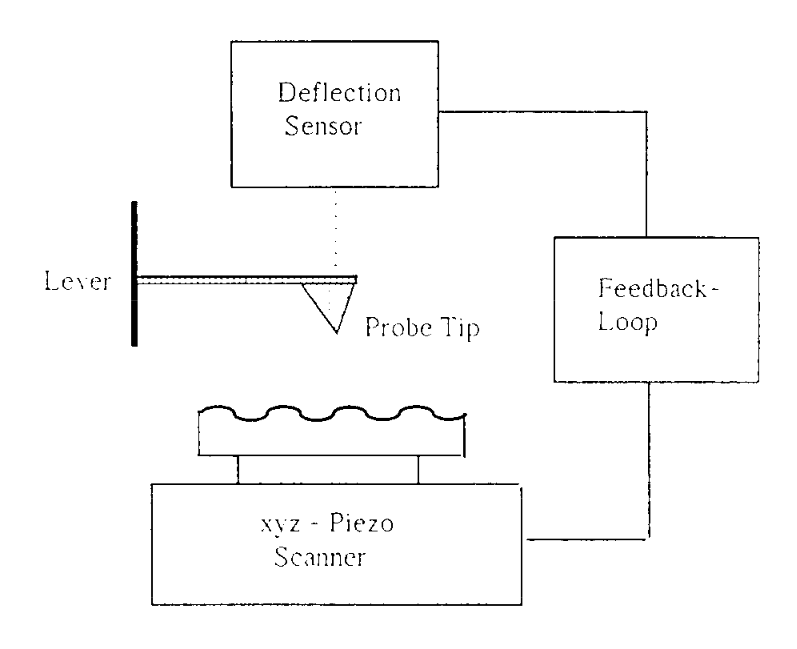
\includegraphics[width = 1\textwidth]{pictures/prinzip.png}
          \caption{asd}
          \label{fig:prinzip}
        \end{figure}
    
        \FloatBarrier


      \subsection{Wechselwirkungen}
        Zur Vermessung des Höhenprofils der Oberfläche wird die distanzabhängige Kraft zwischen Messspitze und Oberfläche genutzt. Das zugehörige Potential wird als Lennard-Jones-Potential 
        
        \begin{equation*}
          \text{U(R)} = 4\text{U}_0 \left[ \left(\frac{\text{R}_{\text{a}}}{\text{r}}\right)^{12} - \left(\frac{\text{R}_{\text{a}}}{\text{r}}\right)^{6} \right]
        \end{equation*}
        
        angenähert, das einen positiven und demnach repulsiven Anteil und einen attraktiven Anteil besitzt, und in Abbildung \ref{fig:LJ} (a) mitsamt der resultierenden Kraft (b) und dem zugehörigen
        Kraftgradienten (c) dargestellt ist.

        \FloatBarrier

        \begin{figure}[h]
          \centering
          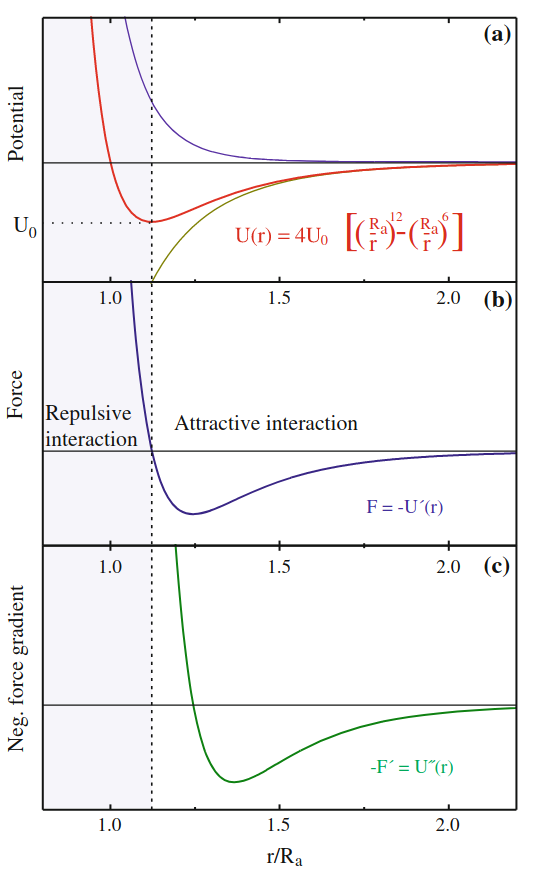
\includegraphics[width = 0.6\textwidth]{pictures/LJ.png}
          \caption{}
          \label{fig:LJ}
        \end{figure}

        \FloatBarrier

        Das Potential setzt sich aus verschiedenen Wechselwirkungen zusammen, die für unterschiedliche Entfernungen dominant sind.\newline 
        Der attraktive Bereich für Abstände über \SI{1}{\nano\metre} resultiert hauptsächlich aus den \textit{Van-der-Waals-Kräften}. Diese beschreiben die Anziehung zweier eigentlich neutraler Atome durch die 
        spontane Entstehung von fluktuierenden Dipolen. Entsteht in einem Atom eine 
        spontaner Dipol, wird im benachbarten Atom ebenfalls ein Dipol induziert und die Atome ziehen sich an. Das zugehörige Potential fällt mit $\frac{1}{\text{r}^6}$ ab und ist demnach langreichweitig. 
        Deswegen wechselwirkt nicht nur das vorderste Atom der Spitze mit der Oberfläche, sondern auch dahinterliegende.\newline

        Für Distanzen unter \SI{1}{\nano\metre} kommt es zu chemischen Bindungen, bei denen die Orbitale der beteiligten Atome hybridisieren. Führt dies zu einer Verringerrung der Gesamtenergie wirken diese 
        Bindungen attraktiv. Erhöht sich die Gesamtenergie wirken die Bindungen repulsiv.

        Für Distanzen unter \SI{1}{\angstrom} kommt es zu stark repulsiven Wechselwirkungen. Die dominante Abstoßung folgt aus dem Pauli-Prinzip, nach dem zwei Elektronen mit dem selben Spin nicht den selben 
        Zustand besetzen dürfen. Bei sehr geringen Distanzen führt der Überlapp der Orbitale dazu, dass Elektronen in höhere unbesetzte Bänder ausweichen müssen. Dies führt zu einer starken Erhöhung der 
        Gesamtenergie und somit zu einer repulsiven Kraft. Zusätzlich kann auch Coulombabstoßung zwischen den Kernen auftreten, wenn diese nicht komplett durch ihre Elektronen abgeschirmt sind.

        \FloatBarrier

        \begin{figure}[h]
          \centering
          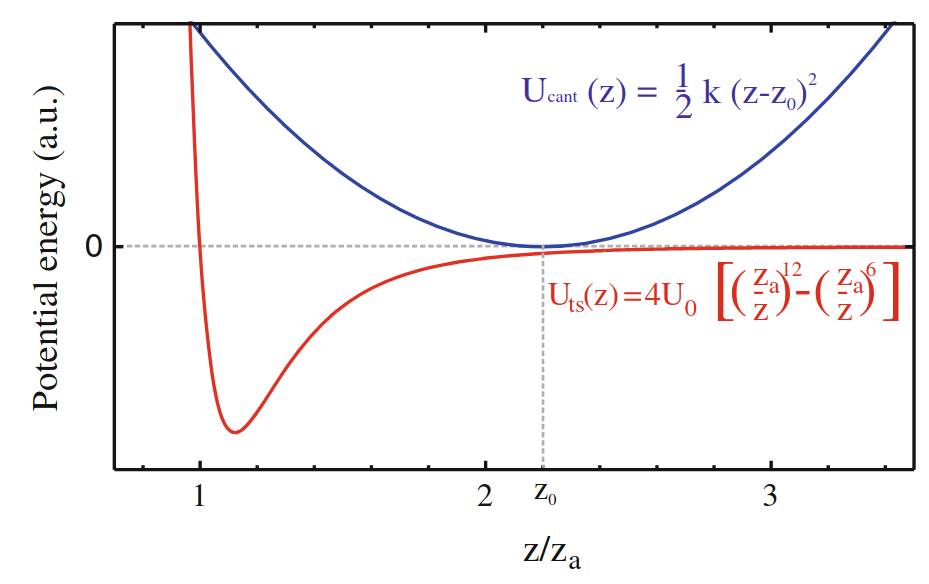
\includegraphics[width = 0.6\textwidth]{pictures/Potentiale.png}
          \caption{}
          \label{fig:Potentiale}
        \end{figure}

        \FloatBarrier


        

      \newpage


      \subsection{Messspitze und Cantilever}
        Um die Intensität der Strahlung in Abhängigkeit der Energie zu messen, wird von einem \textbf{Szintillationsdetektor} in Kombination mit einem \textbf{Diskrimantor} und einem 
        \textbf{Vielkanal-Analysator} Gebrauch gemacht.

        \subsubsection*{Messspitze}
          Das Konzept von Szintillatoren beruht darauf, dass einfallende Strahlung hoher Energie Atome des Szintillationsmediums entweder ionisiert oder anregt und 
          diese beim Relaxieren optische Photonen freisetzen. Die Menge an freigesetzten Photonen hängt dabei von der Energie der einfallenden Strahlung ab. Die optischen Photonen des Relaxationsprozesses 
          werden anschließend von Photomultipliern detektiert. %Grundlegend wird zwischen organischen und anorganischen Szintillatoren unterschieden.
        \newpage
        \subsubsection*{Cantilever}
          Um nur optische Photonen aus dem Szintillationsdetektor zu detektieren wird ein Diskrimantor eingesetzt. Dieser gibt erst ab einem einen Schwellwert übersteigenden Eingangssignal ein Ausgangssignal 
          aus. So kann verhindert werden, dass bereits ein einzelnes spontan emmitiertes Photon einen Ausgangsimpuls am Photomultiplier hervorruft, der fälschlicherweise auf ein optisches Photon des 
          Szintillationsdetektors zurückgeführt werden würde.



      \newpage
      \subsection{Detektionssysteme}
          In diesem Versuch soll die Zusammensetzung von neun Würfeln innerhalb einer 3x3-Würfelebene bestimmt werden. Dazu wird der Würfel aus verschiedenen Richtungen bestrahlt und die transmittierte 
          Intensität gemessen. In eine Richtung i ergibt sich diese zu


      

      \newpage
      \subsection{Messmodi}
          In diesem Versuch soll die Zusammensetzung von neun Würfeln innerhalb einer 3x3-Würfelebene bestimmt werden. Dazu wird der Würfel aus verschiedenen Richtungen bestrahlt und die transmittierte 
          Intensität gemessen. In eine Richtung i ergibt sich diese zu

      
      
      
      \newpage
      \subsection{Piezoelemente}
          In diesem Versuch soll die Zusammensetzung von neun Würfeln innerhalb einer 3x3-Würfelebene bestimmt werden. Dazu wird der Würfel aus verschiedenen Richtungen bestrahlt und die transmittierte 
          Intensität gemessen. In eine Richtung i ergibt sich diese zu



           

